\documentclass{beamer}
\usepackage{booktabs}
\usepackage{pdfpages}
\usepackage{mathtools}
\usepackage{enumerate}
\usepackage{multirow,tabularx}
\usepackage{booktabs}
\usepackage{pdfpages}
\usepackage{proof}
\usepackage{cancel}
\usepackage{chronology}
\usepackage{graphicx}
\usepackage{ulem}
\usepackage{amsmath}
\usepackage{amssymb}
\usepackage{color}
\usepackage{animate}
\usepackage{xr}

\PassOptionsToPackage{usenames,dvipsnames,svgnames}{xcolor}  
\usepackage{tikz}
\usepackage{tkz-graph}


\usepackage{wasysym}
\usepackage{proof}
\usepackage{cancel}
\usepackage{chronology}
\usepackage{graphicx}
\usepackage{ulem}
\usepackage{amsmath}
\usepackage{amssymb}
\usepackage{color}
\usepackage{xcolor}
\usepackage{soul}
%\usepackage{pstricks}
\setbeamertemplate{navigation symbols}{}

\newcommand{\norm}[1]{\left\lVert#1\right\rVert}
\newcommand{\el}{$\mathcal{EL}^{++}$}
\renewcommand{\Re}{\mathbb{R}}
\newcommand{\BigO}[1]{\ensuremath{\operatorname{O}\bigl(#1\bigr)}}
\newcommand{\myul}[2][blue]{\sethlcolor{#1}\hl{#2}\setulcolor{black}}

\newcommand<>{\cunderline}[3]{\only<#1>{#3}\only<#2>{\underline{#3}}}
\newcommand<>{\cem}[3]{\only<#1>{#3}\only<#2>{\ul{#3}}}
\newcommand<>{\cgray}[3]{\only<#1>{#3}\only<#2>{\textcolor{gray}{#3}}}
\newcommand<>{\colorize}[4]{\only<#1>{#4}\only<#2>{\textcolor{#3}{#4}}}

\setbeamertemplate{navigation symbols}{\insertslidenavigationsymbol}
%\setbeamertemplate{navigation symbols}{}
% \addtobeamertemplate{navigation symbols}{}{%
%     \usebeamerfont{footline}%
%     \usebeamercolor[fg]{footline}%
%     \hspace{1em}%
%     \insertframenumber/\inserttotalframenumber
% }

\mode<presentation>
{
\usecolortheme{crane}
%\useoutertheme{split}

\expandafter\def\expandafter\insertshorttitle\expandafter{%
  \insertshorttitle\hfill%
  \insertframenumber\,/\,\inserttotalframenumber}

\usefonttheme[onlysmall]{structurebold}
}
\renewcommand{\em}{\itshape}
\usepackage{pifont}
\definecolor{purple}{rgb}{1,0,1}
\definecolor{dred}{rgb}{0.7,0,0}
\definecolor{myred}{rgb}{1,0,0}
\definecolor{dblue}{rgb}{0,0,0.7}
\definecolor{dgreen}{rgb}{0,0.5,0}
\definecolor{myyellow}{rgb}{1,1,0}
\newcommand{\parents}[1]{parents(#1)}
\setbeamertemplate{itemize item}[ball]


% \mode<presentation>
% {
% \useinnertheme[shadow=true]{rounded}
% \useoutertheme{infolines}
% \usecolortheme{dove}
% \setbeamerfont{block title}{size={}}
% }

\title[Bio-Ontologies]{Semantic similarity and machine learning with ontologies}

\author{Robert Hoehndorf and Maxat Kulmanov}


\date{}

\begin{document}

\begin{frame}
  \titlepage
\end{frame}

\section{Ontologies and graphs}

\begin{frame}
  \frametitle{Preliminaries: ontologies}
  \begin{itemize}
  \item Specific artifacts expressing the intended meaning of a
    vocabulary in terms of primitive categories and relations
    describing the nature and structure of a domain of discourse
    \begin{itemize}
    \item in order to account for the competent use of vocabulary in
      real situations (such as annotations in databases, etc.)
    \end{itemize}
  \item the intended meaning of {\em primitive} categories and
    relations is expressed through axioms (axiomatic method, Tarski)
  \end{itemize}
\end{frame}

\begin{frame}
  \frametitle{Preliminaries: axioms}
  \begin{itemize}
  \item {\em classes} represent kinds of things in the world
    \begin{itemize}
    \item {\em Arm}, {\em Apoptosis}, {\em Influenza}, {\em Homo
        sapiens}, {\em Drinking behavior}, {\em Membrane}
    \end{itemize}
  \item {\em instances} of classes are individuals satisfying the
    classes' intension
    \begin{itemize}
    \item my arm, the influenza I had last year, one ethanol molecule, etc.
    \end{itemize}
  \item {\em relations} between instances arise from interactions,
    configurations, etc., of individuals
    \begin{itemize}
    \item my arm is {\bf part of} me, the {\bf duration of} my
      influenza was 10 days
    \end{itemize}
  \item {\em axioms} specify the conditions that instances of a class
    must satisfy
    \begin{itemize}
    \item every instance of {\em Hand} is a {\bf part of} an instance
      of {\em Arm}
    \end{itemize}
  \end{itemize}
\end{frame}

\begin{frame}
  \frametitle{Description Logics: overview}
  \begin{itemize}
  \item TBox: axioms pertaining to the terminology of the domain (classes)
  \item ABox: axioms stating facts (assertions) about the world
  \item RBox: axioms holding for relations
  \item Reasoning: derive implicitly represented knowledge (e.g.,
    subsumption)
  \item NB: a ``knowledge graph'' is an ABox + RBox
  \end{itemize}
\end{frame}

\begin{frame}
  \frametitle{Manchester OWL Syntax}
  \begin{table}[ht]
    \centering
    \begin{tabular}{|l|l|l|}
      DL Syntax & Manchester Syntax & Example \\
      \hline
      $C \sqcap D$ & C and D & Human and Male \\
      $C \sqcup D$ & C or D & Male or Female \\
      $\neg C$ & not C & not Male \\
      $\exists R.C$ & R some C & hasChild some Human \\
      $\forall R.C$ & R only C & hasChild only Human \\
      $(\geq n R.C)$ & R min n C & hasChild min 1 Human \\
      $(\leq n R.C)$ & R max n C & hasChild max 1 Human \\
      $(= n R.C)$ & R exactly n C & hasChild exactly 1 Human \\
      $\{a\} \sqcup \{b\} \sqcup ...$ & \{a b ...\} & \{John Robert
                                                      Mary\} \\
      \hline
    \end{tabular}
  \end{table}
\end{frame}

\begin{frame}
  \frametitle{Description Logic ALC: syntax}
  \begin{definition}
    Let $N_C$ be a set of concept names and $N_R$ be a set of relation
    names, $N_C \cap N_R = \emptyset$. $\mathcal{ALC}$ concept
    descriptions are inductively defined as:
    \begin{itemize}
    \item If $A \in N_C$, then $A$ is an $\mathcal{ALC}$ concept
      description
    \item If $C, D$ are $\mathcal{ALC}$ concept description, and $r
      \in N_R$, then the following are $\mathcal{ALC}$ concept descriptions:
      \begin{itemize}
      \item $C \sqcap D$
      \item $C \sqcup D$
      \item $\neg C$
      \item $\forall r.C$
      \item $\exists r.C$
      \end{itemize}
    \end{itemize}
  \end{definition}
  \begin{itemize}
  \item Use $\bot$ as abbreviation of $A \sqcap \neg A$, $\top$ as
    abbreviation of $A \sqcup \neg A$
  \end{itemize}
\end{frame}

Examples of concept descriptions, dl1.pdf, p8

\begin{frame}
  \frametitle{Description Logic ALC: semantics}
  \begin{definition}
    An interpretation
    $\mathcal{I} = (\Delta^\mathcal{I}, \cdot^\mathcal{I})$ consists
    of a non-empty domain $\Delta^\mathcal{I}$ and an interpretation
    function $\cdot^\mathcal{I}$:
    \begin{itemize}
    \item $A^\mathcal{I} \subseteq \Delta^\mathcal{I}$ for all $A \in
      N_C$,
    \item $r^\mathcal{I} \subseteq \Delta^\mathcal{I} \times
      \Delta^\mathcal{I}$ for all $r \in N_R$
    \end{itemize}
    The interpretation function is extended to $\mathcal{ALC}$ concept
    descriptions as follows:
    \begin{itemize}
    \item $(C \sqcap D)^\mathcal{I} := C^\mathcal{I} \cap D^\mathcal{I}$
    \item $(C \sqcup D)^\mathcal{I} := C^\mathcal{I} \cup D^\mathcal{I}$
    \item $(\neg C)^\mathcal{I} := \Delta^\mathcal{I} - C^\mathcal{I}$
    \item $(\forall r.C)^\mathcal{I} := \{ d \in \Delta^\mathcal{I} |
      \mbox{for all } e \in \Delta^\mathcal{I}: (d,e) \in
      r^\mathcal{I} \mbox{ implies } e \in C^\mathcal{I}\}$
    \item $(\exists r.C)^\mathcal{I} := \{ d \in \Delta^\mathcal{I} |
      \mbox{there is } e \in \Delta^\mathcal{I}: (d,e) \in
      r^\mathcal{I} \mbox{ and } e \in C^\mathcal{I}\}$
    \end{itemize}
  \end{definition}
\end{frame}

\begin{frame}
  \frametitle{Description Logic: terminologies}
  \begin{itemize}
  \item A concept definition is of the form $A \equiv C$ where
    \begin{itemize}
    \item $A$ is a concept name
    \item $C$ is a concept description
    \end{itemize}
  \item A TBox is a finite set of concept definitions such that it
    \begin{itemize}
    \item does not contain multiple definitions, % A equiv B, A equiv C
    \item does not contain cyclic definitions
      % A equiv B and C, B equiv A and C
    \end{itemize}
  \item A {\em defined concept} occurs on the left-hand side of a
    definition
  \item A {\em primitive concept} does not occur on the left-hand side
    of a definition
    % See: axiomatic-deductive method!
  \item An interpretation $\mathcal{I}$ is a model of a TBox
    $\mathcal{T}$ if it satisfies all its concept definitions:
    $A^\mathcal{I} = C^\mathcal{I}$ for all $A \equiv C \in \mathcal{T}$
  \end{itemize}
\end{frame}

\begin{frame}
  \frametitle{Description Logic: assertions}
  \begin{itemize}
  \item An assertion is of the form $C(a)$ (concept assertion) or
    $r(a,b)$ (role assertion), where $C$ is a concept description, $r$
    is a role, $a,b$ are individual names from a set $N_I$ of such
    names
  \item An ABox is a finite set of assertions
  \item An interpretation $\mathcal{I}$ is a model of an ABox
    $\mathcal{A}$ if it satisfies all its assertions:
    \begin{itemize}
    \item $a^\mathcal{I} \in C^\mathcal{I}$ for all $C(a) \in
      \mathcal{A}$
    \item $(a^\mathcal{I},b^\mathcal{I}) \in r^\mathcal{I}$ for all
      $r(a,b) \in \mathcal{A}$
    \end{itemize}
  \end{itemize}
\end{frame}

\begin{frame}
  \frametitle{Description Logic: Reasoning}
  \begin{itemize}
  \item Subsumption: Is $C$ a subconcept of $D$?
    \begin{itemize}
    \item $C \sqsubseteq_\mathcal{T} D$ iff $C^\mathcal{I} \subseteq
      D^\mathcal{I}$ for all models $\mathcal{I}$ of $\mathcal{T}$
    \end{itemize}
  \item Satisfiability: Is the concept $C$ non-contradictory?
    \begin{itemize}
    \item $C$ is satisfiable w.r.t. $\mathcal{T}$ iff $C^\mathcal{I}
      \not= \emptyset$ for some model $\mathcal{I}$ of $\mathcal{T}$
    \end{itemize}
  \item Consistency: Is the ABox $\mathcal{A}$ non-contradictory?
    \begin{itemize}
    \item $\mathcal{A}$ is consistent w.r.t. $\mathcal{T}$ iff it has
      a model that is also a model of $\mathcal{T}$
    \end{itemize}
  \item Instantiation: Is $e$ an instance of $C$?
    \begin{itemize}
    \item $\mathcal{A} \models_\mathcal{T} C(e)$ iff $e^\mathcal{I}
      \in C^\mathcal{I}$ for all models $\mathcal{I}$ of $\mathcal{T}$
      and $\mathcal{A}$.
    \end{itemize}
  \end{itemize}
\end{frame}

\begin{frame}
  \frametitle{Offtopic: knowledge graphs}
  My favorite definition of ``knowledge graph'':\\
  A knowledge graph is an ABox + RBox.
  \begin{itemize}
  \item ontologies are (mostly) the TBox!
  \end{itemize}
\end{frame}

\begin{frame}
  \frametitle{Ontologies provide background knowledge}
  \centerline{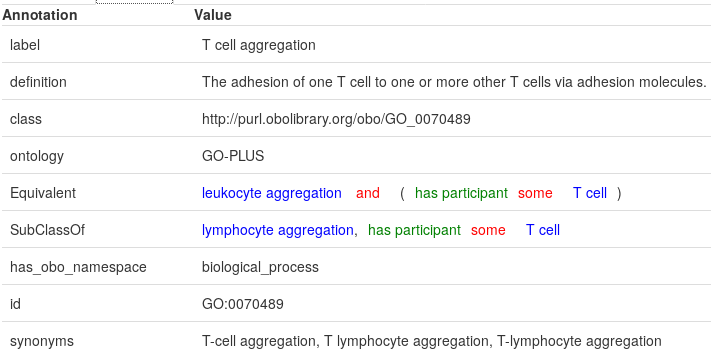
\includegraphics[width=.8\textwidth]{t-cell-aggregation.png}}
\end{frame}

\begin{frame}
  \frametitle{Ontologies provide background knowledge}
  \centerline{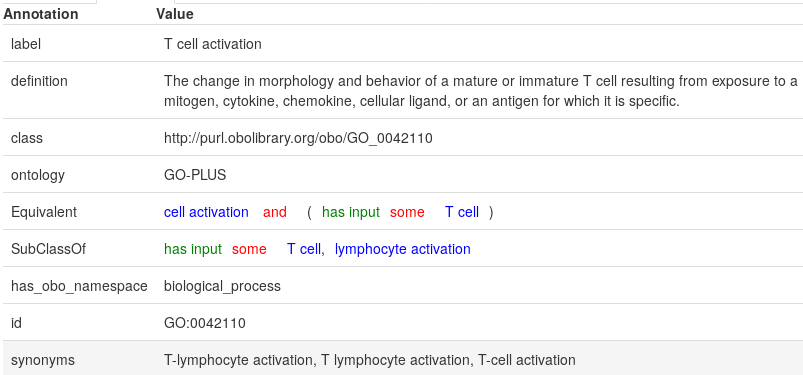
\includegraphics[width=.8\textwidth]{t-cell-activation.png}}
\end{frame}

% \begin{frame}
%   \frametitle{Ontologies provide background knowledge}
%   \centerline{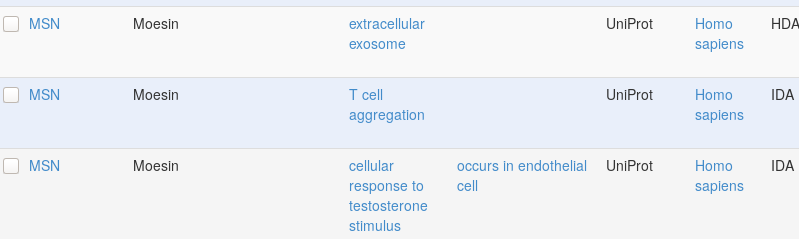
\includegraphics[width=.95\textwidth]{moesin-1.png}}
%   \centerline{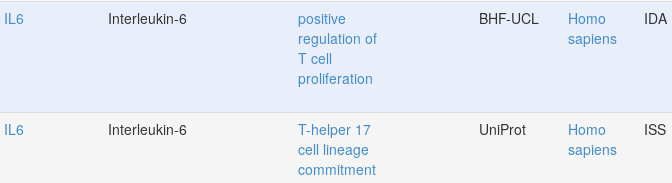
\includegraphics[width=.85\textwidth]{moesin-2.png}}
  
% \end{frame}

\begin{frame}
  \frametitle{Using background knowledge}
  \begin{block}{Problem statement (first attempt):}
    Given a set of entities (instances) within an ontology (DL
    theory). Can we discover/predict {\em new} relations between the
    entities, or between entities and classes in the ontology?
  \end{block}
  \pause
  \begin{itemize}
  \item what relations, and when is a fact ``new''?
  \pause
  \item what features are relevant?
    \begin{itemize}
    \item depends on the relation!
    \end{itemize}
  \pause
  \item finding new facts is only one (minor?) use case
    \begin{itemize}
    \item other uses: encode background knowledge for machine learning
      models; add new classes; expand definition; constrained
      learning; etc.
    \item computing ``similarity''
    \end{itemize}
  \end{itemize}
\end{frame}

\begin{frame}
  \frametitle{Semantic similarity: some examples}
  \begin{itemize}
  \item Are cyclin dependent kinases {\em functionally} more similar
    to lipid kinases or to riboflavin kinases? How about {\em
      phenotypically}?
  \item Which protein in the {\em mouse} is functionally most similar
    to the zebrafish {\em gustducin} protein?
  \item Which mouse knockout resembles {\em Bardet-Biedl Syndrome 8}?
  \item Are there mouse knockouts that resemble the side effects of
    diclofenac?
  \item Which genetic disease produces similar symptoms to ebola?
  \item Does functional similarity correlate with phenotypic
    similarity?
  \end{itemize}
\end{frame}

\begin{frame}
  \frametitle{Semantic similarity}
  semantic similarity measures:
  \begin{itemize}
  \item for words, terms, classes
  \item role of background knowledge:
    \begin{itemize}
    \item statistical/distributional semantics, large corpora
    \item ontologies: (graph) topology
    \end{itemize}
  \item similarity measures: hand-crafted or data-driven?
  \end{itemize}
\end{frame}

\begin{frame}
  \frametitle{Semantic similarity or machine learning}
  \begin{itemize}
  \item semantic similarity measures are mostly hand-crafted
    \begin{itemize}
    \item capture certain intuition about what constitutes
      ``similarity''
    \item different measures for different kinds of similarity
    \item usually interpretable (and explainable)
    \end{itemize}
    \pause
  \item machine learning methods are mostly data-driven
    \begin{itemize}
    \item the architecture of the model is still hand-crafted
    \item usually hard to interpret
    \end{itemize}
  \end{itemize}
\end{frame}

\begin{frame}
  \frametitle{Ontologies and graphs}
  \begin{itemize}
  \item semantic similarity measures {\em and machine learning models} on
    ontologies can be graph-based, feature-based, or model-based
    \begin{itemize}
    \item graph-based: ontology as a graph
    \item feature-based: extract (or obtain) features for
      classes/relations
    \item model-based: define similarity within (special) $\Sigma$-structures
    \end{itemize}
    \pause
  \item we may need to generate graphs from ontologies
    \begin{itemize}
    \item {\em is-a} relations are easy (this is just {\tt owl:subClassOf})
    \item how about {\em part-of}, {\em regulates}, {\em precedes},
      etc.?
    \item disjointness, universal vs. existential quantification,
      cardinality restrictions, intersection, union, negation?
    \end{itemize}
    \pause
  \item relational patterns are implicit in OWL axioms
    \begin{itemize}
    \item design patterns as ``relations'' between classes
    \end{itemize}
  \end{itemize}
\end{frame}

\begin{frame}
  \frametitle{Relations as patterns}
  \centerline{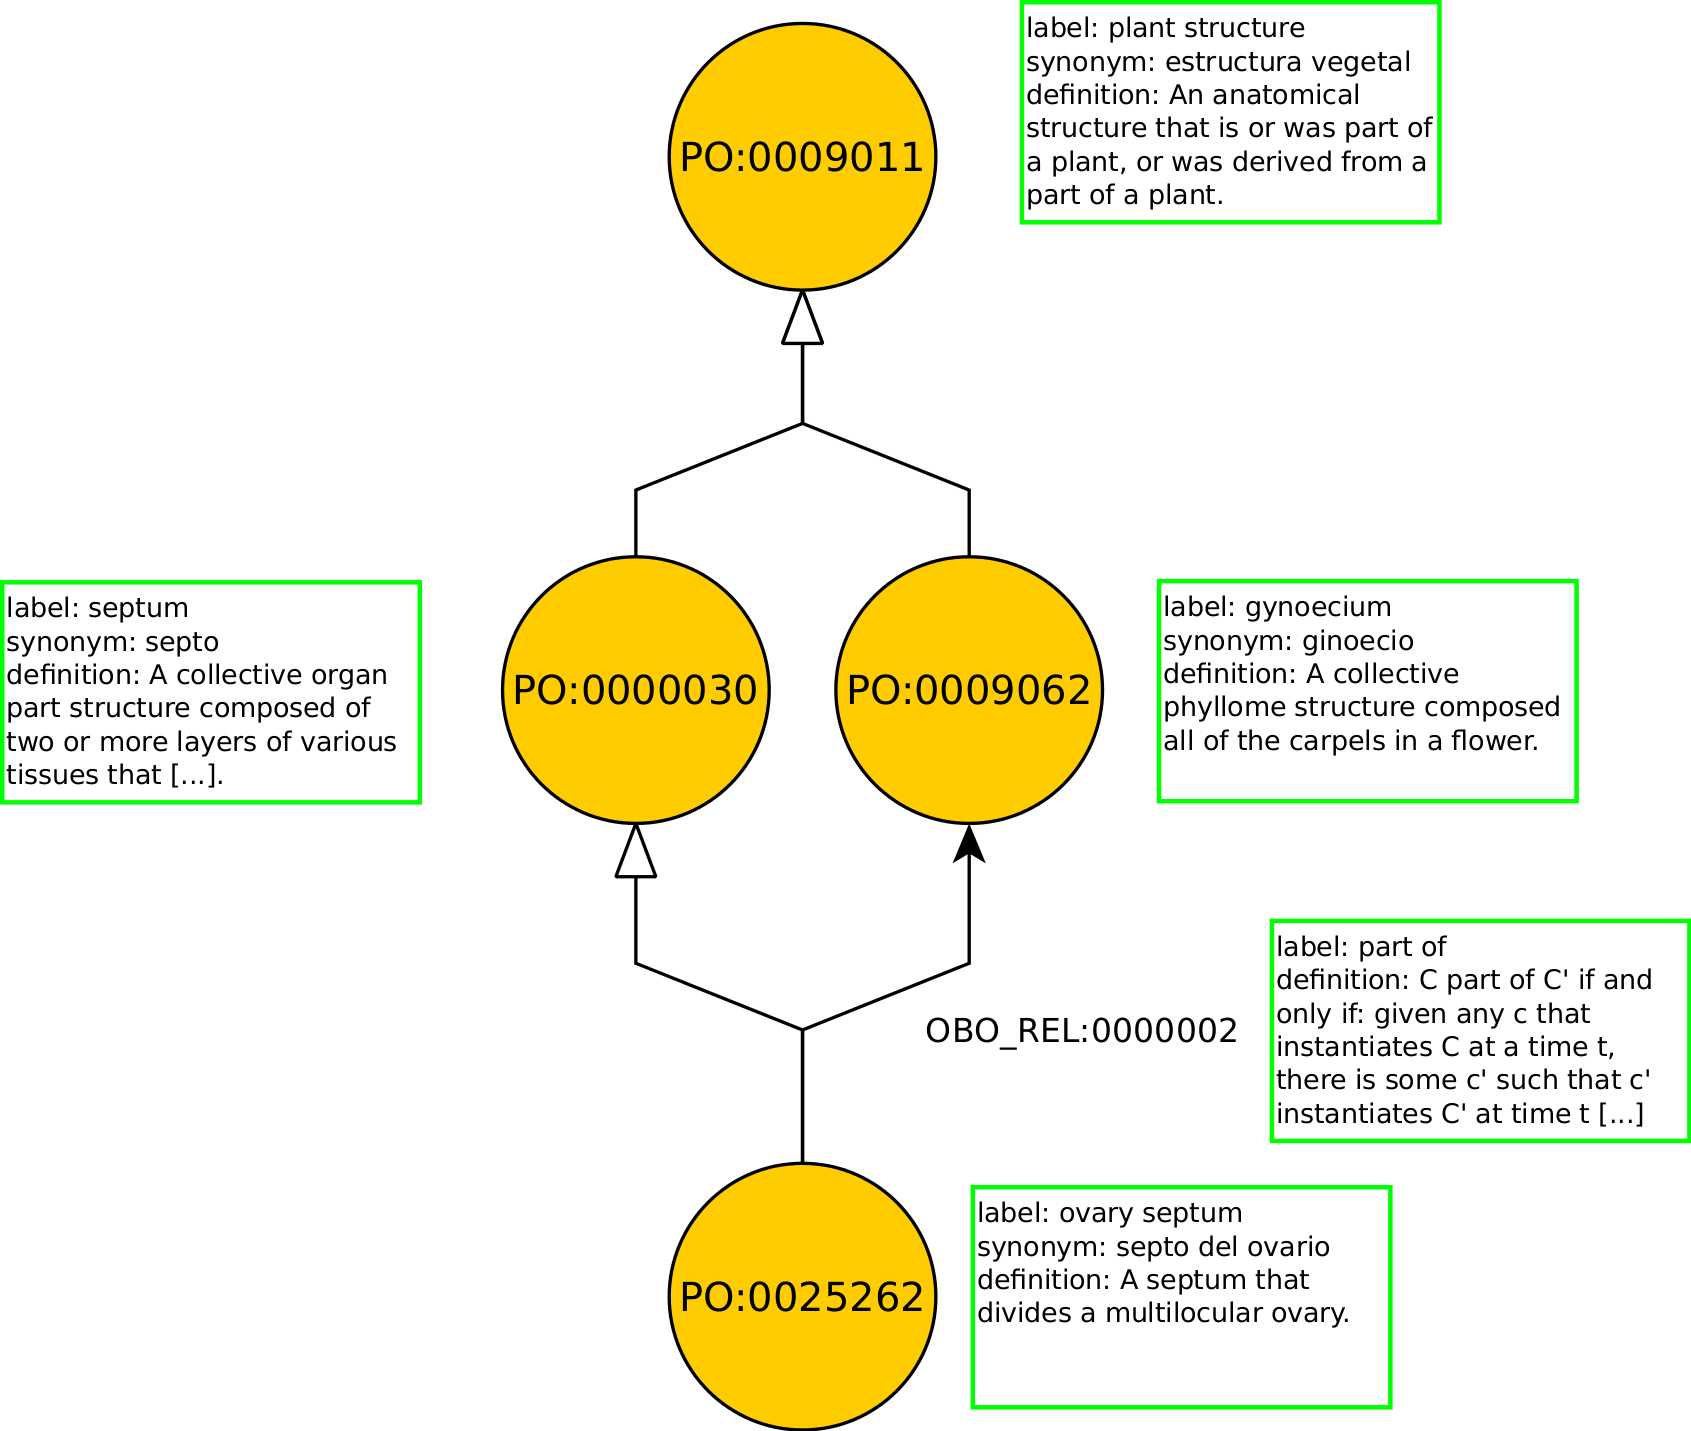
\includegraphics[height=.8\textheight]{plant-ontology-sample.png}}
\end{frame}

% \begin{frame}
%   \frametitle{Relations as patterns}
%   \begin{itemize}
%   \item OBO Relation Ontology (RO):
%     \begin{itemize}
%     \item \url{https://github.com/oborel/obo-relations}
%     \end{itemize}
%   \item Basic Formal Ontology (BFO):
%     \begin{itemize}
%     \item provides top-level classes
%       \begin{itemize}
%       \item Continuant, Process, Function, Material object, etc.
%       \end{itemize}
%     \item used for some OBO Foundry ontologies
%     \end{itemize}
%   \item RO and BFO provide a top-level system of classes and relations
%     shared across many biomedical ontologies
%   \item this system may define patterns used to generate graphs
%   \end{itemize}
% \end{frame}

\begin{frame}
  \frametitle{Relations as patterns}
  \begin{itemize}
  \item {\tt X SubClassOf: Y}: $X \xrightarrow{\text{is-a}} Y$
  \item {\tt X SubClassOf: part-of some Y}: $X \xrightarrow{\text{part-of}} Y$
  \item {\tt X SubClassOf: regulates some Y}: $X \xrightarrow{\text{regulates}} Y$
  \item {\tt X DisjointWith: Y}: $X \xleftrightarrow{\text{disjoint}} Y$
  \item {\tt X EquivalentTo: Y}: $X \xleftrightarrow{\equiv} Y$,
    $\{X,Y\}$
  \item ...
  \end{itemize}
  NB: in bio-ontologies, the OBO Relation Ontology defines these
  patterns
\end{frame}

\begin{frame}
  \frametitle{Asserted and inferred}
  \begin{itemize}
  \item relation patterns can be asserted or inferred
  \item {\tt X SubClassOf: part-of some Y}
  \item {\tt Y SubClassOf: part-of some Z}
  \item {\tt part-of o part-of SubPropertyOf: part-of}
  \item $\vdash$ {\tt X SubClassOf: part-of some Z}
  \item Therefore: $X \xrightarrow{\text{part-of}} Z$
  \item $\Rightarrow$ we should use deductive inference to generate
    these patterns
  \end{itemize}
\end{frame}

\begin{frame}
  \frametitle{Tree models}
  \begin{itemize}
  \item some languages have the {\em finite model} and {\em tree
      model} properties
    \begin{itemize}
    \item such as the Description Logic $\mathcal{ALC}$
    \item generated through a tableaux algorithm
    \end{itemize}
  \item nodes: individuals
    \begin{itemize}
    \item node labels: concept names, concept descriptions
    \end{itemize}
  \item edges: relations between individuals
  \item can be extended to more expressive languages (with blocking,
    cycles, etc.)
  \end{itemize}
\end{frame}

\begin{frame}
  \frametitle{Methods and tools}
  \begin{itemize}
  \item edges should be ``meaningful'': not merely syntax (why?)
    \begin{itemize}
    \item the RDF serialization of OWL is a graph and contains all
      information but is a bad idea for semantic similarity or machine
      learning (more later)
    \item conceptual graphs?
    \end{itemize}
  \item OBO Format represents ontologies as graphs:
    \begin{itemize}
    \item Protege/OWLAPI: OBO export
    \item OBO toolsets (e.g., ROBOT)
    \item
      \url{https://github.com/bio-ontology-research-group/Onto2Graph}
    \end{itemize}
    \pause
  \item but: a conversion of an ontologies into a graph will almost
    always lead to a loss of information
  \end{itemize}
\end{frame}

\end{document}

%%% Local Variables:
%%% mode: latex
%%% TeX-master: t
%%% End:
